%%
%%
%% The first command in your LaTeX source must be the \documentclass command.
\documentclass[sigchi, 12pt, nonacm=true, timestamp=true, screen=true]{acmart}

%%
%% \BibTeX command to typeset BibTeX logo in the docs
\AtBeginDocument{%
  \providecommand\BibTeX{{%
    \normalfont B\kern-0.5em{\scshape i\kern-0.25em b}\kern-0.8em\TeX}}}

%% Rights management information.  This information is sent to you
%% when you complete the rights form.  These commands have SAMPLE
%% values in them; it is your responsibility as an author to replace
%% the commands and values with those provided to you when you
%% complete the rights form.
%%\setcopyright{acmcopyright}
%%\copyrightyear{2018}
%%\acmYear{2018}
%%\acmDOI{10.1145/1122445.1122456}

%% These commands are for a PROCEEDINGS abstract or paper.
%%\acmConference[Woodstock '18]{Woodstock '18: ACM Symposium on Neural
%%  Gaze Detection}{June 03--05, 2018}{Woodstock, NY}
%%\acmBooktitle{Woodstock '18: ACM Symposium on Neural Gaze Detection,
%%  June 03--05, 2018, Woodstock, NY}
%%\acmPrice{15.00}
%%\acmISBN{978-1-4503-9999-9/18/06}


%%
%% Submission ID.
%% Use this when submitting an article to a sponsored event. You'll
%% receive a unique submission ID from the organizers
%% of the event, and this ID should be used as the parameter to this command.
%%\acmSubmissionID{123-A56-BU3}

%%
%% The majority of ACM publications use numbered citations and
%% references.  The command \citestyle{authoryear} switches to the
%% "author year" style.
%%
%% If you are preparing content for an event
%% sponsored by ACM SIGGRAPH, you must use the "author year" style of
%% citations and references.
%% Uncommenting
%% the next command will enable that style.
%%\citestyle{acmauthoryear}

\setcopyright{none}

\usepackage{hyperref}
\usepackage{subfiles}
\usepackage{url}
\usepackage{soul}

%%\citestyle{acmauthoryear}

%%
%% end of the preamble, start of the body of the document source.
\begin{document}

%%
%% The "title" command has an optional parameter,
%% allowing the author to define a "short title" to be used in page headers.
\title{Team 5 Progress Report - MovieEdge}

%%
%% The "author" command and its associated commands are used to define
%% the authors and their affiliations.
%% Of note is the shared affiliation of the first two authors, and the
%% "authornote" and "authornotemark" commands
%% used to denote shared contribution to the research.

\author{Rocko Graziano}
\email{rpgraziano@gatech.edu}
\affiliation{%
  \institution{Georgia Tech OMSCS}
}
\author{Daniel Klass}
\email{dklass3@gatech.edu}
\affiliation{%
	\institution{Georgia Tech OMSCS}
}
\author{Yi Sun}
\email{ysun428@gatech.edu}
\affiliation{%
	\institution{Georgia Tech OMSCS}
}
\author{Jonathan Tay}
\email{jtay6@gatech.edu}
\affiliation{%
	\institution{Georgia Tech OMSCS}
}


%%
%% By default, the full list of authors will be used in the page
%% headers. Often, this list is too long, and will overlap
%% other information printed in the page headers. This command allows
%% the author to define a more concise list
%% of authors' names for this purpose.
%\renewcommand{\shortauthors}{Trovato and Tobin, et al.}

%%
%% The abstract is a short summary of the work to be presented in the
%% article.
\begin{abstract}
	We present \textbf{MovieEdge}, a recommendation system which provides an interactive visualization interface for users.
\end{abstract}
%%
%% The code below is generated by the tool at http://dl.acm.org/ccs.cfm.
%% Please copy and paste the code instead of the example below.
%%
%%\begin{CCSXML}
%%<ccs2012>
%% <concept>
%%  <concept_id>10010520.10010553.10010562</concept_id>
%%  <concept_desc>Computer systems organization~Embedded systems</concept_desc>
%%  <concept_significance>500</concept_significance>
%% </concept>
%% <concept>
%%  <concept_id>10010520.10010575.10010755</concept_id>
%%  <concept_desc>Computer systems organization~Redundancy</concept_desc>
%%  <concept_significance>300</concept_significance>
%% </concept>
%% <concept>
%%  <concept_id>10010520.10010553.10010554</concept_id>
%%  <concept_desc>Computer systems organization~Robotics</concept_desc>
%%  <concept_significance>100</concept_significance>
%% </concept>
%% <concept>
%%  <concept_id>10003033.10003083.10003095</concept_id>
%%  <concept_desc>Networks~Network reliability</concept_desc>
%%  <concept_significance>100</concept_significance>
%% </concept>
%%</ccs2012>
%%\end{CCSXML}

%%\ccsdesc[500]{Computer systems organization~Embedded systems}
%%\ccsdesc[300]{Computer systems organization~Redundancy}
%%\ccsdesc{Computer systems organization~Robotics}
%%\ccsdesc[100]{Networks~Network reliability}

%%
%% Keywords. The author(s) should pick words that accurately describe
%% the work being presented. Separate the keywords with commas.
%%\keywords{movies, DVA, lorem ipso}

%% A "teaser" image appears between the author and affiliation
%% information and the body of the document, and typically spans the
%% page.
%%\begin{teaserfigure}
%%  \includegraphics[width=\textwidth]{sampleteaser}
%%  \caption{Seattle Mariners at Spring Training, 2010.}
%%  \Description{Enjoying the baseball game from the third-base
%%  seats. Ichiro Suzuki preparing to bat.}
%%  \label{fig:teaser}
%%\end{teaserfigure}

%%
%% This command processes the author and affiliation and title
%% information and builds the first part of the formatted document.
\maketitle

\section{Introduction}
Recommender Systems (RS) are ubiquitous in modern digital life. A fruitful area of RS research has been movie ratings, where a database of ratings drives Collaborative Filtering (CF) to suggest new movies to watch. Interest in movie CF models peaked in 2007 with \href{https://www.netflixprize.com/}{The Netflix Prize}. However, CF models are complex and hard for users to interpret.

Recently, researchers have introduced MovieExplorer \cite{taijala2018movieexplorer}, which allows users to navigate a latent high (30) dimensional space derived from user preference data (“taste space”) to find movies they may be in the mood to watch. 

\subsection{Innovation}

We introduce MovieEdge, which extends on MovieExplorer in two key ways.  We will augment exploration by visualizing the taste space as the user explores, providing supplemental data drawn from other data sources \cite{openMovieDB} along the way. Interpretability  \cite{Molnar2019interpretable} can assist with user acceptance, detecting bias, and satisfy users’ curiosity. 

We will enhance MovieExplorer’s accuracy  by using a more powerful RS. Specifically, we will use a Word2vec model \cite{mikolov2013distributed} to build the RS. As shown in \cite{ozsoy2016word}, this can increase CF model performance while leading to latent vector representations that are visually intuitive \cite{mikolov2013distributed}. 

\section{Related Work}
\subsection{Collaborative Filtering Recommender Systems}

Early CF systems were driven by nearest-neighbor similarity methods \cite{herlocker1999algorithmic}, \cite{smith2017two}, weighting similarity between user vectors of ratings. While neighborhood-based CF are easy to implement, they are not as accurate as more complex models.

Item-based CF methods are driven by item-to-item similarity. Amazon constructed a similar-items table by finding items that people tend to buy together \cite{linden2003amazon}, \cite{smith2017two}. Scalability is achieved via offline pre-processing. However, they focus on real-time performance and sacrifice user-centric interpretability. 

The Netflix Prize introduced new CF algorithms based on matrix factorization (MF) \cite{funk2006netflix}. User-item ratings are viewed as a matrix where rows represent users and columns movies: ratings are the sparse matrix entries. MF seeks to estimate unknown ratings by approximating the ratings matrix with a low-rank decomposition. MF is highly accurate for movie rating prediction, and it remains the predominant CF technique today \cite{koren2008factorization}. 

One shortcoming of MF is that only user-item ratings are taken into account. Rendle \cite{rendle2012factorization} developed Factorization Machines (FM), a supervised learning algorithm that models feature interactions with factorized parameters.  FMs can be seen as a generalization of MF which can easily incorporate side-channel features along with user-item ratings matrix for greater accuracy while reducing training time.

Vector representation of words (Word2vec) is widely adopted in Natural Language Processing (NLP). Two  architectures, Continuous Bag-of-Words (CBOW) and Skim-gram models \cite{mikolov2013efficient},  \cite{mikolov2013distributed}, \cite{rong2014word2vec} were introduced to learn embeddings from words in sentences. The embeddings capture contextual similarity. This can be applied to user-item interaction data by treating items as words and the set of items rated highly by each user as a sentence \cite{ozsoy2016word}. Training Word2vec takes advantage of one-hot-encoding (OHE). However, movie ratings are often not binary, increasing architectural complexity.

\subsection{Interactive Recommendations}

Most RS are not interactive. MetaLens \cite{schafer2002meta} gives users session-specific control over the recommendation process, improving user satisfaction. MetaLens is limited to filtering or sorting the list of recommendations with user-specified criteria. The potential filters are hard-coded and reflect user constraints rather than content preferences. 

MovieExplorer \cite{taijala2018movieexplorer}, which incorporates user feedback in the RS, is closest to MovieEdge. MovieExplorer allows the user to navigate the model's latent factor space by expressing their session-specific preferences for movies.  As the session progresses, MovieExplorer presents better recommendations. MovieExplorer’s interactive exploration paradigm increased user satisfaction. However, MovieExplorer asks users to navigate the high dimensional latent factor space without a visual reference. 

\subsection{Visualization of Embedding Spaces}

t-Stochastic Neighbor Embedding \mbox{t-SNE} \cite{maaten2008visualizing} projects high dimensional feature vectors into 2D visualizations. \mbox{t-SNE} computes similarity scores between observations in the high dimensional feature space and finds a low dimensional embedding: points which are close in high dimensional space remain close in the projected space. \mbox{t-SNE} is nonlinear and adaptive to the data distribution. \mbox{t-SNE} is known for producing high-quality visualizations, albeit at the cost of hyperparameter tuning and computation. Using \mbox{t-SNE} can be difficult, and much care must be taken with interpretation \cite{wattenberg2016how}.

Taking the gradient of the \mbox{t-SNE} cost function with respect to the coordinates in the embedding space can be compute expensive.  Acceleration \mbox{t-SNE} through tree-based algorithms like the Barnes-Hut approximation \cite{van2014accelerating} can help to “summarize” observations.  

Embedding Projector \cite{smilkov2016embedding} leverages \mbox{t-SNE} to visualize high dimensional data. We will adopt this approach in the high dimensional taste space of our CF model, augmenting with supplemental data and user interactivity. 

Our primary dataset is MovieLens \cite{harper2016movielens}, which includes over 27,000 unique movies. Ward Hierarchical clustering \cite{ward1963hierarchical} will reduce the visual load:  its hierarchical nature will allow users to zoom in and out of the visualization as we dynamically expand and collapse the clusters.

\subsection{Evaluating Recommender Systems}

RS has traditionally been evaluated on accuracy. Herlocker \cite{herlocker2004evaluating} proposed an alternative metric, Serendipity, the tendency for a RS to produce  “interesting” recommendations. By visualizing the latent CF model space during exploration, MovieEdge greatly increases the chance of a serendipitous encounter.

\section{Building the Similarity Model}

\textit{Introduce this section}

\subsection{Preparing the Data}

We have gathered the data from MovieLens \cite{harper2016movielens} and the Open Movie Database \cite{openMovieDB}. 

\textit{Jonathan}

\subsection{Word2Vec}

\textit{Daniel \& Yi}

\subsection{Matrix Factorization}

\textit{Jonathan}

\section{Visualizing Recommendations}

\textit{Rocko, ???}

\section{Updated Project Plan}

\textit{describe remaining tasks \& any challenges}

\section{Results}

\textit{describe testing plan}

\section{Conclusions}

\textit{what have we learned thus far}

%\section{Project Overview}
%\subfile{sections/today}
%\subfile{sections/novelty}
%\subfile{sections/audience}
%\subfile{sections/difference-impact}
%
%\section{Project Details}
%\subfile{sections/risks-payoff}
%\subfile{sections/costs}	
%\subfile{sections/projectplan}
%\section{Conclusion}
%\subfile{sections/conclusion}

%% the bibliography file.


%\bibliographystyle{apalike}
\bibliographystyle{ACM-Reference-Format}
\bibliography{bibliography}

%
%\begin{figure*}
%	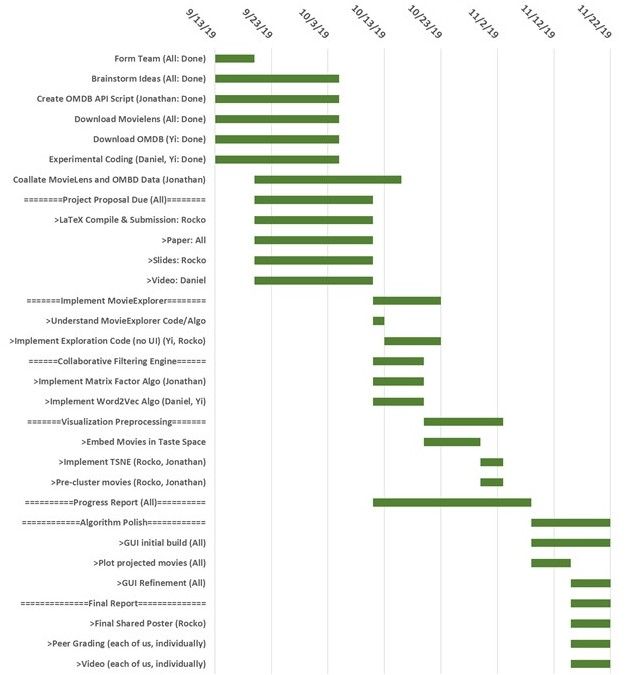
\includegraphics{ProjectPlan}
%	\caption{Project Plan}
%	\label{fig:ProjectPlan}
%\end{figure*}

%\begin{figure*}
%	\centering
%	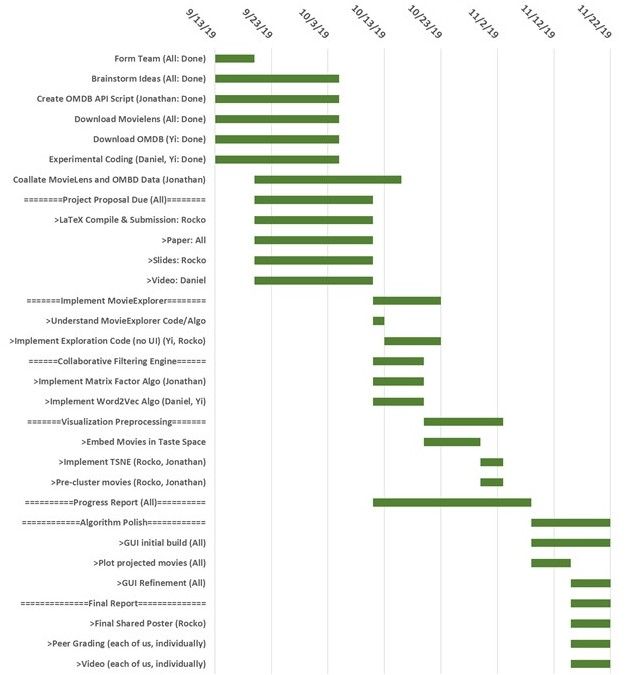
\includegraphics[width=1\linewidth]{ProjectPlan}
%	\caption[Project Plan]{Plan of Activities-Work shared equally among all team members}
%	\label{fig:projectplan}
%\end{figure*}


\end{document}
\endinput

%%
%% End of file `sample-sigconf.tex'.
